
\documentclass[letterpaper, reqno,11pt]{article}
\usepackage[margin=1.0in]{geometry}
\usepackage{color,latexsym,amsmath,amssymb}
\usepackage{graphicx}

\newcommand{\RR}{\mathbb{R}}
\newcommand{\CC}{\mathbb{C}}
\newcommand{\ZZ}{\mathbb{Z}}
\newcommand{\QQ}{\mathbb{Q}}
\newcommand{\NN}{\mathbb{N}}
\begin{document}
\pagenumbering{arabic}
\title{Selected Exercise Solutions for The Art Of Computer Programming}
\author{Yuchong Pan}
\date{\today}
\newtheorem{thm}{Theorem}
\maketitle
%

\section{Basic Concepts}

\subsection{Algorithms}

\begin{enumerate}
    \item[5.] The procedure fails to be a genuine algorithm for the following three points:
    \begin{itemize}
        \item \emph{Finiteness.} After one finishes all the 12 chapters, the procedure suggests starting from Chapter 1.
        \item \emph{Output.} The procedure does not have outputs.
        \item \emph{Effectiveness.} It is unclear whether each step can be completed in a finite amount of time. For instance, there are open problems in the exercises which no one knows the solution.
    \end{itemize}
    The procedure has the following differences in format between it and Algorithm E:
    \begin{itemize}
        \item The procedure does not include a paragraph specifying the inputs and the purpose (outputs) of the procedure.
        \item Each step of the procedure does not have a phrase that briefly summarizes the principal content of the step.
    \end{itemize}
    \item[7.] Let $n \in \NN$. If $n > m$, then after E1, $r = m \neq 0$. Therefore, in E3, $m$ and $n$ are essentially exchanged. This reduces to the definition of $T_m$. Since $T_m$ is well-defined, then so is $U_m$, and $U_m = T_m + 1$.
    \item[9.] We say that ``$C_2$ is a representation of $C_1$'' or ``$C_2$ simulates $C_1$'' if
    \begin{itemize}
        \item there exists $\delta : Q_1 \to 2^{Q_2}$ such that for all $q_1, q_2 \in Q_1$ with $q_1 \neq q_2$, $\delta\left(q_1\right) \cap \delta\left(q_2\right) = \emptyset$;
        \item for all $q \in Q_1$ and $q' \in \delta(q)$, there exist $n \in \NN$ and $q_1', \ldots, q_n' \in Q_2$ such that
        \begin{align*}
            q_1' &= f_2\left(q'\right), \\
            q_{i + 1}' &= f_2\left(q_i'\right), && \forall i = 1, \ldots, n - 1, \\
            q_n' &\in \delta\left(f_1(q)\right).
        \end{align*}
    \end{itemize}
\end{enumerate}

\subsection{Mathematical Preliminaries}

\subsubsection{Mathematical Induction}

\begin{enumerate}
    \item[8.]
    \begin{enumerate}
        \item If $n = 1$, then $1^3 = 1$.
        
        Let $n \geq 1$. Suppose by induction that $n^3 = (2(1 + \ldots + (n - 1)) + 1) + (2(1 + \ldots + (n - 1) + 1)) + \ldots + (2(1 + \ldots + n - 1) + 1)$. Then
        \begin{align*}
            (n + 1)^3 &= n^3 + 3n^2 + 3n + 1 \\
            &= (2(1 + \ldots + (n - 1)) + 1) + (2(1 + \ldots + (n - 1) + 1) + 1) + \ldots \\
            &\quad + (2(1 + \ldots + n - 1) + 1) + 3n^2 + 3n + 1 \\
            &= (2(1 + \ldots + (n - 1)) + 1 + 2n) + (2(1 + \ldots + (n - 1) + 1) + 1 + 2n) + \ldots \\
            &\quad + (2(1 + \ldots + n - 1) + 1 + 2n) + 3n^2 + 3n + 1 - 2n \cdot n \\
            &= (2(1 + \ldots + n) + 1) + (2(1 + \ldots + n + 1) + 1) + \ldots \\
            &\quad + (2(1 + \ldots + (n + 1) - 2) + 1) + n^2 + 3n + 1 \\
            &= (2(1 + \ldots + n) + 1) + (2(1 + \ldots + n + 1) + 1) + \ldots \\
            &\quad + (2(1 + \ldots + (n + 1) - 2) + 1) + \left(2 \cdot \frac{n^2 + 3n}{2} + 1\right).
        \end{align*}
        It remains to show that $1 + \ldots + (n + 1) - 1 = \frac{n^2 + 3n}{2}$. We have
        \begin{align*}
            1 + \ldots + (n + 1) - 1 &= \frac{(1 + (n + 1)) \cdot (n + 1)}{2} - 1 \\
            &= \frac{(n + 1)(n + 2)}{2} - 1 \\
            &= \frac{n^2 + 3n + 2}{2} - 1 \\
            &= \frac{n^2 + 3n}{2}.
        \end{align*}
        This completes the proof.
        \item Adding up $1^3, 2^3, \ldots, n^3$ and applying (a),
        \begin{align*}
            1^3 + 2^3 + \ldots + n^3 &= 1 + 3 + 5 + \ldots + (2(1 + \ldots + n) - 1) \\
            &= \frac{(1 + (2(1 + \ldots + n) - 1)) \cdot (1 + \ldots + n)}{2} \\
            &= \frac{2(1 + \ldots + n)^2}{2} \\
            &= (1 + \ldots + n)^2.
        \end{align*}
    \end{enumerate}
    \item[13.] See Figure \ref{fig:1.2.1-13}.
    \begin{figure}[h]
        \centering
        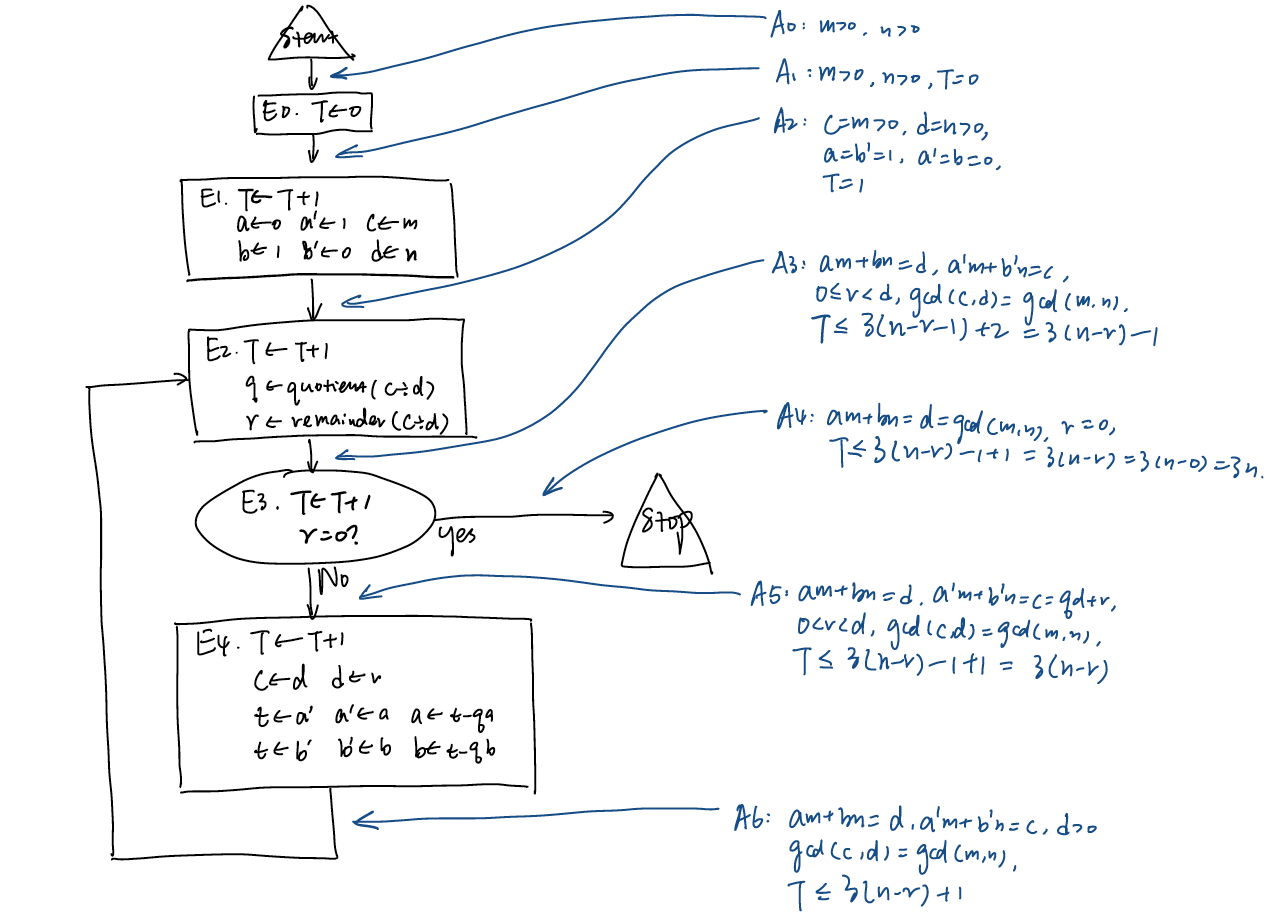
\includegraphics[width=\textwidth]{figures/fig_1-2-1_13.png}
        \caption{Flow chart for Algorithm E with assertions that prove $T \leq 3n$.}
        \label{fig:1.2.1-13}
    \end{figure}
    \item[15.]
    \begin{enumerate}
        \item Suppose for the sake of contradiction that $\ZZ$ is well-ordered by $<$. Since $\ZZ \subseteq \ZZ$, then by (iii) there exists $x \in \ZZ$ with $x \leq y$ for all $y \in \ZZ$. Note that $x - 1 \in \ZZ$ and that $x - 1 < x$. By (ii), $x \leq x - 1$ is not true, a contradiction. This completes the proof.
        \item Define $f : \ZZ \to \NN$ by
        $$ f(x) = \left\{
            \begin{array}{ll}
                1, & x = 0, \\
                2x, & x > 0, \\
                -2x + 1, & x < 0,
            \end{array}
        \right. \qquad x \in \ZZ. $$
        Define $x \prec y$ oif $f(x) < f(y)$ for all $x, y \in \ZZ$. We show that $\ZZ$ is well-ordered by $\prec$.
        \begin{enumerate}
            \item[i)] Let $x, y, z \in \ZZ$. Suppose that $x \prec y$ and that $y \prec z$. Then $f(x) < f(y)$ and $f(y) < f(z)$. Thus, $f(x) < f(z)$. By the definition of $\prec$, $x \prec z$.
            \item[ii)] Let $x, y \in \ZZ$. Then existly one of the following tree possibilities is true: $f(x) < f(y)$, $f(x) = f(y)$, or $f(y) < f(x)$.

            If $f(x) < f(y)$, then $x \prec y$. If $f(y) < f(x)$, then $y \prec x$. Suppose that $f(x) = f(y)$. If $f(x) = f(y) = 1$, then $x = y = 0$. If $f(x) = f(y)$ is even, i.e. $f(x) = f(y) = 2k$ for some $k \in \NN$, then $x = y = k$ by the definition of $f$. If $f(x) = f(y)$ is odd and not equal to $1$, i.e. $f(x) = f(y) = 2k + 1$ for some $k \in \NN$, then $f(x) = f(y) = -2(-k) + 1$. By the definition of $f$, $x = y = -k$. In either case, $x = y$.

            Hence, exactly one of the following three possibilities is true: $x \prec y$, $x = y$, or $y \prec x$.
            \item[iii)] Let $A \subseteq Z, A \neq \emptyset$. Then there exists $a_0 \in A$. Suppose for the sake of contradiction that there does not exist $x \in A$ such that $x \preceq y$ for all $y \in A$. Thus, for all $x \in A$, there exists $y \in A$ such that $y \prec x$. Therefore, there exists $a_1 \in A$ such that $a_1 \prec a_0$. By the definition of $\prec f\left(a_1\right)  < f\left(a_0\right)$. Having defined $a_1, \ldots, a_k$, there exists $a_{k + 1} \in A$ such that $f\left(a_{k + 1}\right) < f\left(a_k\right)$.

            Let $B = \left\{ f\left(a_k\right) : k \in \ZZ, k \geq 0 \right\} \subseteq \NN$. Since $\NN$ is well-ordered by $<$, then there exists $x = f\left(a_j\right) \in B$ for some $j \in \ZZ, j \geq 0$ such that $x \leq y$ for all $y \in B$. However, $f\left(a_{j + 1}\right) \in B$ and $f\left(a_{j + 1}\right) < f\left(a_j\right)$, a contradiction. This completes the proof.
        \end{enumerate}
        \item No. Suppose for the sake of contradiction that $[0, \infty)$ is well-ordered by $<$. Since $(0, \infty) \subseteq [0, \infty)$, then by (iii), there exists $x \in (0, \infty)$ such that $x \leq y$ for all $y \in (0, \infty)$. Note that $\frac{x}{2} \in (0, \infty)$ and that $\frac{x}{2} < x$. By (ii), $x \leq \frac{x}{2}$ is not true, a contradiction. This completes the proof.
        \item Yes.
        \begin{enumerate}
            \item[i)] Let $x = \left(x_1, \ldots, x_n\right), y = \left(y_1, \ldots, y_n\right), z = \left(z_1, \ldots, z_n\right) \in T_n$. Suppose that $x \prec y$ and that $y \prec z$. This implies that there exists $k_1, 1 \leq k_1 \leq n$ such that $x_j = y_j$ for $1 \leq j < k_1$ and that $x_{k_1} \prec y_{k_1}$, and that there exists $k_2, 1 \leq k_2 \leq n$ such that $y_j = z_j$ for $1 \leq j < k_2$ and that $y_{k_2} \prec z_{k_2}$. Let $k = \min\left(k_1, k_2\right)$. Let $j \in \NN$ with $1 \leq j < k = \min\left(k_1, k_2\right)$. Then $1 \leq j < k_1$ and $1 \leq j < k_2$. Thus, $x_j = y_j$ and $y_j = z_j$, so $x_j = z_j$.

            Without loss of generality, assume that $k = k_1$. Then $k_1 \leq k_2$. Thus, $x_k = x_{k_1} \prec y_{k_1}$. If $k_1 < k_2$, then $y_{k_1} = z_{k_1} = z_k$ and hence $x_k \prec z_k$. If $k_1 = k_2$, then $y_{k_1} = y_{k_2} \prec z_{k_2} = z_{k_1} = z_k$ and by (i), $x_k \prec z_k$. By the definition of $\prec$ on $T_n$, $x \prec z$.
            \item[ii)] Let $x = \left(x_1, \ldots, x_n\right), y = \left(y_1, \ldots, y_n\right) \in T_n$. If $x_k = y_k$ for all $1 \leq k \leq n$, then $x = y$. Otherwise, there exists $k \in \NN, 1 \leq k \leq n$ such that $x_k \neq y_k$. Let $k^*$ be the smallest such $k$. Then $x_j = y_j$ for all $1 \leq j < k$. Since $S$ is well-ordered by $\prec$, then either $x_k \prec y_k$, or $y_k \prec x_k$. By the definition of $\prec$, either $x \prec y$, or $y \prec x$, respectively.
            \item[iii)] Let $A \subseteq T_n$. Let $A_1 = \left\{ x_1 \in S : \left(x_1, \ldots, x_n\right) \in A \right\} \subseteq S$. Since $S$ is well-ordered by $\prec$, then there exists $x_1^* \in A_1$ such that $x_1^* \preceq y_1$ for all $y_1 \in A_1$. Having defined $x_1^*, \ldots, x_k^*$ for $1 \leq k < n$, let $A_{k + 1} = \left\{ x_{k + 1} \in S : \left(x_1^*, \ldots, x_k^*, x_{k + 1}, \ldots, x_n\right) \in A \right\} \subseteq S$. Since $S$ is well-ordered by $\prec$, then there exists $x_{k + 1}^* \in A_{k + 1}$ such that $x_{k + 1}^* \preceq y_{k + 1}$ for all $y_{k + 1} \in A_{k + 1}$.

            Let $x^* = \left(x_1^*, \ldots, x_n^*\right)$. Let $y = \left(y_1, \ldots, y_n\right) \in A$. We show that $\left(x_1^*, \ldots, x_n^*\right) \preceq \left(y_1, \ldots, y_n\right)$. Suppose for the sake of contradiction that this is not true. Then by (ii), $y \prec x^*$. By the definition of $\prec$, there exists $k \in \NN, 1 \leq k \leq n$ such that $y_k \prec x_k^*$. This however contradicts that $x_k^*  \preceq y_k$. This completes the proof.
        \end{enumerate}
        \item No. Let $A = \{ (1), (0, 1), (0, 0, 1), (0, 0, 0, 1), \ldots \} \subseteq T$. Clearly $A \neq \emptyset$. Suppose for the sake of contradiction that there exists $x \in A$ such that $x \preceq yy$ for all $y \in A$. By the definition of $A$, there exists $k \in \ZZ, k \geq 0$ such that $x = (\underbrace{0, \ldots, 0}_\text{$k$ $0$'s}, 1)$. Note that $(\underbrace{0, \ldots, 0}_\text{$(k + 1)$ $0$'s}, 1) \in A$ and that by the definition of $\prec$, $(\underbrace{0, \ldots, 0}_\text{$(k + 1)$ $0$'s}, 1) \prec (\underbrace{0, \ldots, 0}_\text{$k$ $0$'s}, 1) = x$, a contradiction. This completes the proof.
        \item ($\Longrightarrow$) Suppose that $S$ is well-ordered by $\prec$. By the definition of well-ordering, $\prec$ satisfies (i) and (ii). Suppose for the sake of contradiction that there exists an infinite sequence $x_1, x_2, x_3, \ldots$ with $x_{j + 1} \prec x_j$ for all $j \geq 1$. Let $A = \left\{ x_1, x_2, \ldots \right\} \subseteq S$. Clearly $A \neq \emptyset$. Since $S$ is well-ordered by $\prec$, then there exists $x \in A$ such that $x \preceq y$ for all $y \in A$. Suppose that $x = x_k$ for some $k \in \NN$. Note that $x_{k + 1} \in A$ and that $x_{k + 1} \prec x_k$, a contradiction. This completes the proof.

        ($\Longleftarrow$) Suppose that $\prec$ satisfies (i) and (ii), and that there exists no infinite sequence $x_1, x_2, \ldots$ with $x_{j + 1} \prec x_j$ for all $j \geq 1$. Suppose for the sake of contradiction that $S$ is not well-ordered by $\prec$. Since $\prec$ satisfies (i) and (ii), then $\prec$ does not satisfy (iii). Thus, there exists $A \subseteq S, A \neq \emptyset$ such that for all $x \in A$, there exists $y \in A$ such that $y \prec x$. Since $A \neq \emptyset$, then there exists $x_0 \in A$. Having defined $x_0, \ldots, x_k \in A$, since $x_k \in A$, then there exists $x_{k + 1} \in A$ such that $x_{k + 1} \prec x_k$. This defines an infinite sequence $x_0, x_1, \ldots$ with $x_{j + 1} \prec x_j$ for all $j \geq 1$, a contradiction. This completes the proof.
        \item Suppose that $P(x)$ can be proved under the assumption that $P(y)$ is true for all $y \prec x$. Suppose for the sake of contradiction that there exists $x \in S$ such that $P(x)$ is false. Let $A = \{ x \in S : \text{$P(x)$ is false} \} \subseteq S$. Then $A \neq \emptyset$. Since $S$ is well-ordered by $\prec$, then there exists $x^* \in A$ such that $x^* \preceq y$ for all $y \in A$. Let $z \prec x^*$. Then $P(z)$ is true. For otherwise $z \in A$ and hence $x^* \preceq z$, a contradiction by (ii). This shows that $P(z)$ is true for all $z \in x^*$. By the assumption, $P\left(x^*\right)$ can be proved to be true, a contradiction. This completes the proof.
    \end{enumerate}
\end{enumerate}

\end{document}